\documentclass[12pt,a4paper]{article}
\usepackage[utf8]{inputenc}
\usepackage[english]{babel}
\usepackage{listings}
\usepackage{xcolor}
\usepackage{graphicx}
\usepackage{geometry}
 \geometry{
 a4paper,
 total={170mm,257mm},
 left=25mm,
 top=20mm,
 right=25mm,
 bottom=20mm
 }

\title{\bf Cube of a Number using 8051}
\author{\vspace{-10ex}}
\date{\vspace{-10ex}}
\begin{document}
\maketitle

\begin{minipage}{0.45\textwidth}
        \begin{tabular}{l l}
            \textbf{Expt No:}&13\\
            \textbf{Date :}&23/10/2020
        \end{tabular}
\end{minipage}%
\begin{minipage}{0.45\textwidth}
        \begin{tabular}{l l}
             \textbf{Name:}& Shivanirudh S G  \\
             \textbf{Reg No:} & 185001146 
        \end{tabular}
\end{minipage}
\vspace{1cm}
\hrule
\begin{flushleft}
\subsection*{\textbf{Aim:}} 
To find the cube of a number using \textbf{8051 microcontroller}.

\subsubsection*{\textbf{Algorithm:}}
\begin{itemize}
    \item Move hex value 00 to register 0. 
    \item Move the value of register 1 to A and B.
    \item Multiply A and B using MUL AB to get $A^2$.
    \item Move value of register 1 to B and again perform MUL AB to get $A^3$. 
    \item The higher and lower bits stored in B and A should be moved to R4 and R5 respectively.
\end{itemize}

\newpage
\subsubsection*{\textbf{Program:}}

\begin{table}[htb]
\centering
\begin{tabular}{|l|l|} 
\hline
\textbf{Program}                                                 & \textbf{Comments}                             \\ 
\hline
\hline
mov r0, \#00                                                     & Move hex value 00 to Register 0               \\
\hline
mov a, r1                                                        & Move value in Register 1 to A                 \\
\hline
mov b, r1                                                        & Move value in Register 1 to B                 \\
\hline  
mul ab                                                           & A = A * B                                     \\
\hline
mov b, r1                                                        & Move value in Register 1 to B                 \\
\hline
mul ab                                                           & A = A * B                                     \\
\hline
mov r4, b                                                        & Move value of B into Register 4               \\
\hline
mov r5, a                                                        & Move value of A into Register 5               \\
\hline
here:~sjmp here                                                  & Halt                                          \\
\hline
\end{tabular}
\end{table}

\subsubsection*{\textbf{Input and Output:}}
\begin{figure}[h]
    \centering
    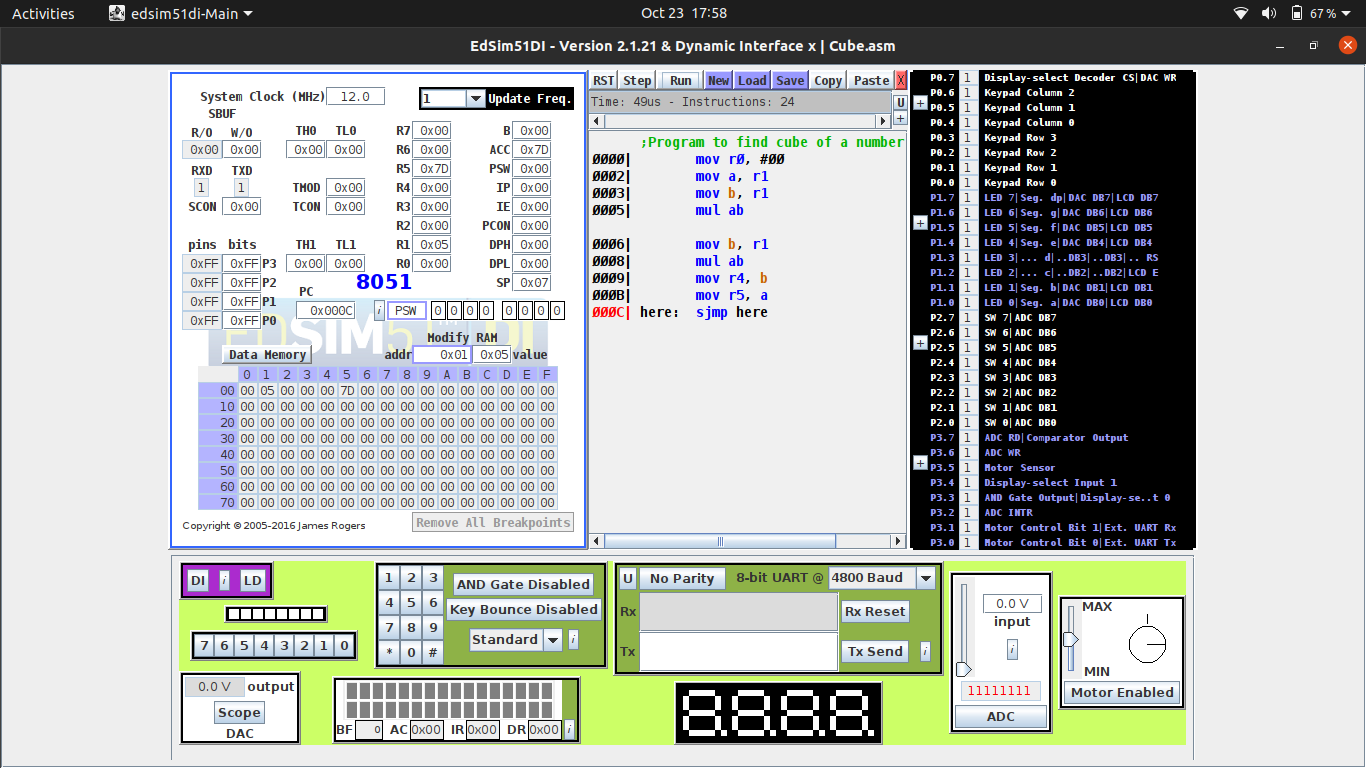
\includegraphics[trim = 60mm 75mm 60mm 10mm, clip, width = \textwidth]{Pics/Cube.png}
    \caption{ \textbf{Input:} r1: 05h; 
              \textbf{Output:} Higher: 00h, Lower: 7Dh}
\end{figure}
\hrule
\subsection*{\textbf{Result:}}
The 8051 program to cube a number was written, and the results observed.
\end{flushleft}
\end{document}